\documentclass[12pt]{article}
\usepackage{sbc-template}
\usepackage{graphicx}
\usepackage{amsmath}
%\usepackage{subfigure}
%\usepackage{times,amsmath,epsfig}
%\usepackage{graphicx,url}
 \makeatletter
 \newif\if@restonecol
 \makeatother
 \let\algorithm\relax
 \let\endalgorithm\relax 
\usepackage[lined,algonl,ruled]{algorithm2e}
\usepackage{multirow}
\usepackage[brazil]{babel}
\usepackage[utf8]{inputenc}  

\sloppy

\title{TRABALHO PRÁTICO 1: \\ Máquina Virtual}

\author{Pedro Lopes Miranda Junior}

\address{Departamento de Ciência da Computação -- Universidade Federal de Minas Gerais (UFMG)
\email{plmj@dcc.ufmg.br}
}

\begin{document}
\maketitle

\begin{resumo} 
Este trabalho constitui na implementação de uma máquina básica capaz de
executar um código passado em linguagem de máquina.
\end{resumo}

\section{Introdução}
\label{introducao}
Ao longo do curso serão estudados diversos conceitos sobre liguagem de máquina.
Perante isso, serão dados diversos trabalhos que testarão alguns dos inúmeros
conceitos abordados.

O primeiro trabalho tem como objetivo implementar o simulador para uma máquina
virtual básica, capaz de decodificar algumas funções simples. Esse trabalho é
de extrema importância pois a partir dele todos os demais trabalhos serão
executados.

A máquina virtual é constituída de registradores de uso geral, uma memória de
no mínimo 1024 espaços, e registradores de uso especial e todas essas estruturas
são capazes de endereçar o tamanho de um inteiro (4 bytes).

Ao todo a máquina virtual pode decodificar 23 funções, divididas em acesso à
memória, operações lógicas, aritmeticas e saltos, condicionais ou não).

\section{Solução Proposta}
\label{solucao_proposta}
Para solucionar o problema, foi criada uma estrutura de dados que chamada vm
(Virtual Machine), que contem a memória, os registradores e outras ifnofrmações
adicionais, como está descrita abaixo.

\subsection{Estruturas de dados}

\subsubsection{VM}

\begin{algorithm}[h!]
\begin{footnotesize}
   \textbf{mem[MEMSIZE],m,fmem;} \textit{Memória, endereços de memória disponíveis e
   endereço de memória final} \\
   \textbf{pc,sp,fp;} \textit{Registradores especificos: PC,SP e FP} \\
   \textbf{reg[4];} \textit{Registradores de uso geral: reg[0]=RA, reg[1]=RB, reg[2]=RB
   e reg[3]=RD}\\
   \textbf{rflags[2];} \textit{Registradores de flag:
   rflags[0]=zero,rflags[1]=negativo}\\
   \textbf{char mode;} \textit{Carácter que indica o modo de impressão do código}\\
\caption{Estrutura da máquina virtual}
\end{footnotesize}
\end{algorithm}

\subsection{Algoritmos}

Foram implementadas algumas funções que auxiliam no funcionamento da máquina
virtual, portanto todas as funções operam sobre o tipo VM.

\subsubsection{Funções}
\begin{algorithm}[h!]
\begin{footnotesize}
   \textbf{initialize;} \textit{Inicialisa a máquina virtual com os parâmetros
   passados} \\
   \textbf{readmem;} \textit{Faz a leitura do programa para a memória} \\
   \textbf{exec;} \textit{Executa a máquina virtual} \\
   \textbf{getinst;} \textit{Busca a próxima instrução a ser executada} \\
   \textbf{decode;} \textit{Decodifica e executa a instrução buscada} \\
   \textbf{incpc;} \textit{Incrementa o registrador PC} \\
   \textbf{verbose;} \textit{Imprime as informações quando no modo verbose} \\

\caption{Funções da máquina virtual}
\end{footnotesize}
\end{algorithm}


\section{Implementação}
\label{implementacao}
Na implementação do problema proposto foram tomadas várias decisões, dentre
elas criar um tipo de dados para a máquiva virtual, dividir o código em funções
de modo que na função principal fique o menor conteúdo possível ajudando no
encapsulamento do código e em futuras manutenções e melhorias.

Foi decidido criar um tipo de dados para a máquina virtual pois esse tipo de
disposição facilita a adição futura de demais estruturas na máquina virtual.
Além disso o acesso ao TAD é feito de maneira melhor estruturada e o
encapsulamento é melhor feito.

A divisão do código em funções ajuda no encapsulamento do TAD, e na melhor
modularização do mesmo.

\subsection{Código}
O código foi dividido em arquivos \textit{.c} e \textit{.h} que estão listados
abaixo

\subsubsection{Arquivos .c}
\begin{itemize}
\item \textbf{vm.c:} Contém a função principal da máquina virtual;
\item \textbf{vmdata.c:} Contém as funções do tipo VM;
\end{itemize}

\subsubsection{Arquivos .h}

\begin{itemize}
\item \textbf{vmdata.h:} Contém as definições das funções do tipo VM
\end{itemize}

\subsection{Compilação}

O programas deve ser compilado através de um makefile, chamando \textit{vm}
ou através do compilador GCC chamando:\\

\begin{footnotesize}
\begin{verbatim} gcc -Wall vm.c vmdata.c -o vm \end{verbatim}
\end{footnotesize}

\subsection{Execução}

Para a execução do programa deverão ser recebidos,impreterívelmente, como parâmetros o valor
inicial do PC, valor inicial - tamanho - do SP, posição de memória inicial, o
modo de saída - S ou V - dos dados e o nome do arquivo com o código a ser
executado.

O comando para execução do programa é da forma: \\

\begin{footnotesize}
\begin{verbatim} ./vm 10 250 5 <modo> <arquivo> \end{verbatim}
\end{footnotesize}

\subsubsection{Formato da entrada}
O arquivo de entrada citado deverá ser um programa em linguagem de máquina,
onde cada linha conterá uma instrução, como abaixo:

\begin{footnotesize}
\begin{verbatim}
01
30
90
01
30
11
00
25
11
01
24
42
01
00
\end{verbatim}
\end{footnotesize}

\subsubsection{Formato da saída}
O formato da saída depende da especificação do modo de execução do programa.\\
Em modo simples, o programa apenas imprimirá os comandos de impressão na saída
padrão, já em modo verbose a forma de impressão será após cada instrução, tendo
cada linha os valores de cada um dos parametro, como consta no exemplo abaixo:

\begin{footnotesize}
\begin{verbatim}
INST: XX; PC: XX; SP: XX; FP: XX; 
Flag.Zero: X; Flag.Neg: X; RA: XX; 
RB: XX; RC: XX; RD: XX;
\end{verbatim}
\end{footnotesize}

\section{Avaliação Experimental}
\label{avaliacao_experimenta}
O programa foi executado e testado numa máquina rodando o sistema baseado em
debian Linux Mint. A máquina em questão tem uma memória de 8GB e um processador
Core I7 de 2.2GHz.

Foram feitos vários testes de execução do programa,onde todas as funções
testadas funcionaram de maneira rápida e sem erro. Abaixo apresentamos imagens
da execução do programa e sua saída em modo verbose para um dos testes criados.

\begin{figure}[h!]
\centering
 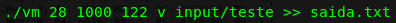
\includegraphics[scale=0.5]{./img/exec.png}
   \caption{Comando de execução do programa}
\end{figure}

\begin{figure}[h!]
\centering
 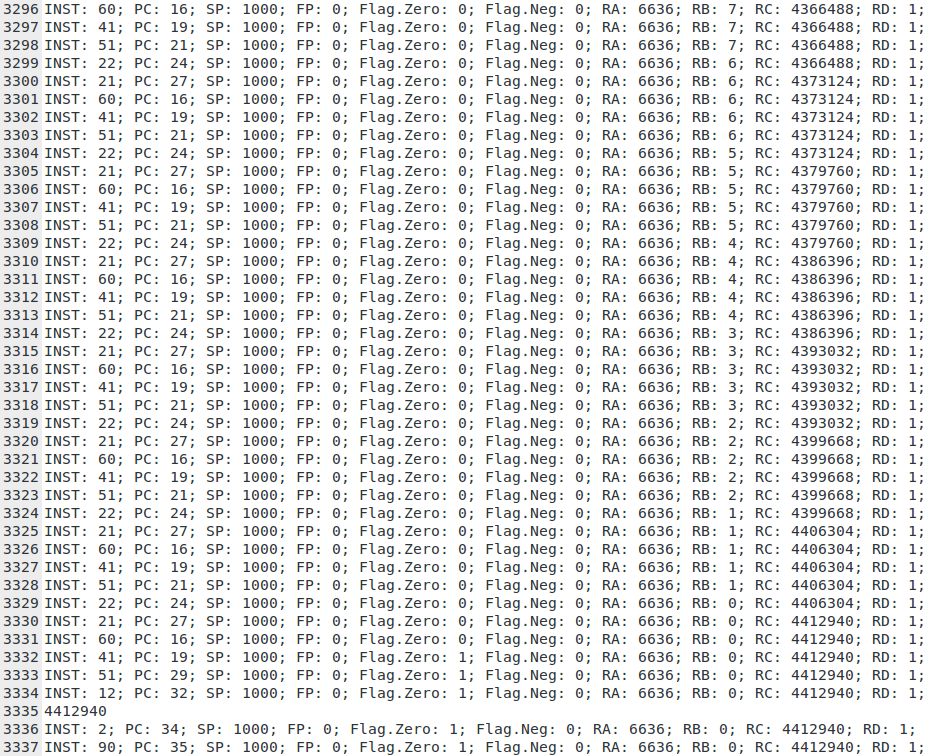
\includegraphics[scale=0.5]{./img/teste.png}
 \caption{Saída usando verbose}
\end{figure}

\section{Conclusão}
\label{conclusao}
O trabalho correu sem grandes problemas, sendo a parte mais difícil o
entendimento do funcionamento de algumas funções, pois qualquer coisa errada
poderá influenciar totalmente os demais trabalhos da disciplina.

O programa atendeu a diversos valores de entrada e creio que a solução proposta
atenda ao especificado

\end{document}
